\documentclass[aps, prl, letterpaper, twocolumn, superscriptaddress, notitlepage, 10pt]{revtex4-1}
\usepackage{times}

% use these settings for a more reader-friendly version
%\documentclass[aps, pra, a4paper, 11pt, onecolumn, nofootinbib, superscriptaddress, tightenlines, notitlepage, longbibliography]{revtex4-1}

%------------------------------------------------------------------------------------------------------------%
% Packages
%------------------------------------------------------------------------------------------------------------%

\usepackage{color}
\usepackage{amsmath,amsfonts,amssymb}
\usepackage{graphicx}
\usepackage[caption=false]{subfig}
\usepackage{enumerate}

\usepackage{tikz}
\usetikzlibrary{arrows,decorations.pathmorphing,backgrounds,positioning,fit,shapes.misc}

\usepackage{epstopdf} % to include .eps graphics files with pdfLaTeX
%\usepackage{bm}  % Define \bm{} to use bold math fonts

\usepackage[pdfpagelabels,pdftex,bookmarks,breaklinks]{hyperref}
\definecolor{darkblue}{RGB}{0,0,127} % choose colors
\definecolor{darkgreen}{RGB}{0,150,0}
\hypersetup{colorlinks, linkcolor=darkblue, citecolor=darkgreen, filecolor=red, urlcolor=blue}
\hypersetup{pdfauthor={Simon Burton, Courtney Brell, Steven T. Flammia}}
%\hypersetup{pdftitle={Title\ Goes\ Here}}

%------------------------------------------------------------------------------------------------------------%
% Macros
%------------------------------------------------------------------------------------------------------------%

\newcommand{\Eref}[1]{Eq.~(\ref{#1})}
\newcommand{\Fref}[1]{Fig.~\ref{#1}}

\newcommand{\e}{\mathrm{e}}

\newcommand{\ket}[1]{|{#1}\rangle}
\newcommand{\expect}[1]{\langle{#1}\rangle}
\newcommand{\bra}[1]{\langle{#1}|}
\newcommand{\ketbra}[2]{\ket{#1}\!\bra{#2}}
\newcommand{\braket}[2]{\langle{#1}|{#2}\rangle}
\newcommand{\proj}[1]{\ketbra{#1}{#1}}

%------------------------------------------------------------------------------------------------------------%
% Comment fonts
%------------------------------------------------------------------------------------------------------------%

\newcommand{\cggb}[1]{\textcolor{blue}{#1}}
\newcommand{\dude}[1]{\textcolor{red}{#1}}
\newcommand{\stf}[1]{\textcolor{green}{#1}}

%------------------------------------------------------------------------------------------------------------%
\begin{document}

\title{Classical Simulation of Quantum Error Correction in a Fibonacci Anyon Code}

\author{Simon Burton}
\affiliation{Centre for Engineered Quantum Systems, School of Physics, 
The University of Sydney, Sydney, Australia}
\author{Courtney G.\ Brell}
\affiliation{Institut f\"{u}r Theoretische Physik, Leibniz Universit\"{a}t Hannover, 
Appelstra\ss{}e 2, 30167 Hannover, Germany}
\author{Steven T.\ Flammia}
\affiliation{Centre for Engineered Quantum Systems, School of Physics, 
The University of Sydney, Sydney, Australia}

\date{\today}

\begin{abstract}
Classically simulating the dynamics of excitations in two-dimensional quantum systems that 
support anyons is likely intractable in general because such dynamics are sufficient to implement 
universal quantum computation. However, processes of interest for the study of quantum 
error correction in anyon systems are typically drawn from a restricted class that displays 
significant structure over a wide range of system parameters.
We exploit this structure to classically simulate, and thereby demonstrate the success of, an 
error-correction protocol for a quantum memory based on the universal Fibonacci anyon 
model.  We numerically simulate a phenomenological model of the system and noise 
processes on lattice sizes of up to 
$128\times128$ sites, and find a lower bound on the error-correction threshold of 
approximately $12.5\%$, which is comparable to those previously known for abelian and 
(non-universal) nonabelian anyon models.
\end{abstract}

\maketitle

%------------------------------------------------------------------------------------------------------------%

Topologically ordered quantum systems in two dimensions show tremendous promise for 
long-term storage and processing of quantum information~\cite{Kitaev2003, Dennis2002, Nayak2008}. 
The topological features of such systems are insensitive to local 
perturbations~\cite{Bravyi2010, Bravyi2011a, Michalakis2013}, and have quasiparticle excitations 
exhibiting anyonic statistics~\cite{Wilczek1990}. These systems can in general be used as 
quantum memories~\cite{Kitaev2003, Dennis2002} or to perform universal topological 
quantum computation~\cite{Freedman2002, Nayak2008}.

Quantum error correction is vital to harnessing the computational power of topologically 
ordered systems. When coupled to a heat bath at any finite temperature, thermal fluctuations 
will create spurious anyons that diffuse and quickly corrupt the stored quantum 
information~\cite{Pastawski2010}. Thus, the passive protection provided by the mass gap 
at low temperature must be augmented by an \emph{active} decoding procedure. 

In order to efficiently classically simulate an error-correction protocol for a topologically ordered quantum memory, it is necessary to simulate the physical noise processes, the decoding algorithm, and the physical recovery operations. Decoding algorithms are typically designed to run efficiently on a classical computer, but there is generally no guarantee that the noise and recovery processes should be classically simulable.
Because of this, almost all of the sizable research effort on active quantum error correction for topological systems has focused on the case of abelian anyons~\cite{Dennis2002, Duclos-Cianci2010, Duclos-Cianci2010a, Wang2010, Wang2010a, Duclos-Cianci2013, Bravyi2011, Bombin2012, Wootton2012, Anwar2014, Watson2014, Hutter2014a, Bravyi2014, Wootton2015, Fowler2015, Andrist2015}.
%~\cite{Dennis2002, Duclos-Cianci2010, Bravyi2011, Bravyi2014}.
Systems of abelian anyons are well suited to studying quantum error correction because (at the RG fixed point) noise and recovery processes can be efficiently simulated numerically, allowing lattice simulations of decoding with over 1 million sites~\cite{Duclos-Cianci2010}. 
Standard algorithms are specifically tailored to exploit the abelian nature of these particles, particularly that abelian anyons cannot be used for quantum computation. 

Recent investigations have begun to explore quantum error correction for nonabelian anyon 
models~\cite{Brell2013, Wootton2013, Hutter2014}. Nonabelian anyon models are especially interesting 
because braiding and fusion of these anyons in general allows for the implementation of universal quantum 
computation. However, the initial studies of error-correction in nonabelian anyon systems have focused on specific models, such as the Ising 
anyons~\cite{Brell2013} and the so-called $\Phi$-$\Lambda$ 
model~\cite{Wootton2013, Hutter2014} that, while nonabelian, are not universal. The general dynamics of these particular anyon models is known to be efficiently classically simulable, a fact
that was exploited to enable efficient simulation of error correction in these systems. When considering more general anyon models, their ability to perform universal quantum computation would seem a significant barrier to their simulation on a classical computer. While simulation of general dynamics does indeed seem intractable, we argue that the kinds of processes that are typical of thermal noise are sufficiently structured to allow for their classical simulation in the regimes where we expect successful error correction to be possible. This insight allows us to simulate the noise and recovery processes for a quantum code based on a universal anyon model.

Concretely, we consider the simulation of quantum error correction in a two-dimensional lattice 
system with Fibonacci anyons, a class of nonabelian anyons that are universal for quantum 
computation~\cite{Freedman2002, Nayak2008}. Fibonacci anyons are experimentally motivated as the 
expected excitations of the $\nu=\frac{12}{5}$ fractional quantum Hall 
states~\cite{Slingerland2001}, and can also be realized in several spin 
models~\cite{Levin2005, Bonesteel2012, Kapit2013, Palumbo2014} and composite 
heterostructures~\cite{Mong2014}.

We use a flexible phenomenological model of dynamics and thermal noise to describe a system with Fibonacci anyon excitations. Within this model, we apply existing general topological error-correction protocols, and simulate the successful preservation of quantum information encoded in topological degrees of freedom. Topological quantum computation protocols using nonabelian anyons typically implicitly assume the existence of an error-correction protocol to correct for diffusion or unwanted creation of anyons. Our results are the first explicit demonstration that such a scheme will be successful when applied to a universal topological quantum computer.

%------------------------------------------------------------------------------------------------------------%
\paragraph{Modeling Fibonacci anyons.}

The topological features of a physical anyon model are abstractly described by a unitary 
modular tensor category~\cite{Wang2010b}. This object contains the data describing the 
types of anyonic particles, as well as the results of topological operations such as braiding and 
fusion of these anyons. The Fibonacci anyon model consists of only one non-trivial particle 
type, conventionally labelled $\tau$. Denoting the vacuum by $\mathbb{I}$, we can describe 
the possible fusion outcomes of Fibonacci anyons as $\tau\times\tau=\mathbb{I}+\tau$, 
i.e.~two $\tau$ particles can either fuse to vacuum or to a $\tau$ particle.

Associated with each set of fusion outcomes for a fixed number of $\tau$ particles is a basis 
vector for a Hilbert space, the \emph{fusion} space. For $n$ particles of type $\tau$, the 
dimension of this space grows asymptotically as $\varphi^n$ for $\varphi=\frac{1+\sqrt{5}}{2}$ 
the golden ratio. Additionally, there is a global degeneracy associated with the topology of the 
manifold on which the anyons reside. We will consider systems with the topology of a torus, 
which for the Fibonacci anyons gives rise to a 2-fold degeneracy. For convenience 
(in particular to minimize finite-size effects in our numerical computations~\cite{Brell2013}), 
this global space is the one in which we will encode, and demonstrate protection of, quantum 
information.

The fusion outcome of any particular experiment depends on the history of the particles, in 
particular how they have braided around one another. Braiding operations are treated as 
unitary actions on the fusion space. Pair-creation events should be considered isometries 
that enlarge the fusion space, while fusion events correspond to projective measurements 
of combined charge of some number of particles. For detailed description of these 
processes in Fibonacci anyons, see e.g.~Ref.~\cite{Nayak2008} and references therein. 
Braiding of Fibonacci anyons and measurements of fusion outcomes is known to be 
sufficient to implement universal quantum computation~\cite{Freedman2002, Nayak2008}.

The dynamics and history of a system of anyons can be conveniently represented by a graphical calculus, which can be regarded as a representation of the world-lines of the particles. These diagrams can be manipulated by $R$-moves, corresponding to braiding processes:
	\begin{align}
		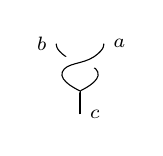
\begin{tikzpicture}[baseline=0.5cm,scale=0.3]		
			\draw(0,0)--(0,1);
			\draw plot [smooth, tension=1] coordinates { (0,1) (0.75,1.8) (-0.6,2.45) (-1,3)};
			\draw[color=white, line width=7] plot [smooth, tension=1] coordinates { (0,1) (-0.75,1.8) (0.6,2.45) (1,3)};
			\draw plot [smooth, tension=1] coordinates { (0,1) (-0.75,1.8) (0.6,2.45) (1,3)};
			\node at (0,0) [anchor=west] {{\scriptsize $c$}};
			\node at (-1,3) [anchor=east] {{\scriptsize $b$}};
			\node at (1,3) [anchor=west] {{\scriptsize $a$}};
		\end{tikzpicture}
		&\;\;=\;\;R^{ab}_c\cdot\;
		\begin{tikzpicture}[baseline=0.5cm,scale=0.3]		
			\draw(0,0)--(0,1);
			\draw(0,1)--(-1,2)--(-1,3);
			\draw(0,1)--(1,2)--(1,3);
			\node at (0,0) [anchor=west] {{\scriptsize $c$}};
			\node at (-1,3) [anchor=east] {{\scriptsize $b$}};
			\node at (1,3) [anchor=west] {{\scriptsize $a$}};
		\end{tikzpicture}
	\end{align}
where $a$, $b$, and $c$ represent particle types, or $F$-moves, representing the associativity rule for fusion processes, denoted as
	\begin{align}
		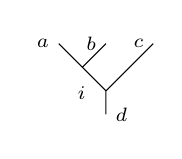
\begin{tikzpicture}[baseline=0.6cm,scale=0.3]
			\draw(0,0)--(0,1)--(-2,3);
			\draw(0,3)--(-1,2);
			\draw(2,3)--(0,1);
			\node at (-0.45,1.6) [anchor=north east] {{\scriptsize $i$}};
			\node at (0,0) [anchor=west] {{\scriptsize $d$}};
			\node at (2,3) [anchor=east] {{\scriptsize $c$}};
			\node at (0,3) [anchor=east] {{\scriptsize $b$}};
			\node at (-2,3) [anchor=east] {{\scriptsize $a$}};
		\end{tikzpicture}
		&\;\;=\;\;\sum_j[F^{abc}_d]_{ij}\cdot\;
		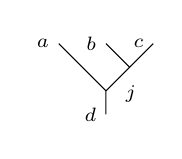
\begin{tikzpicture}[baseline=0.6cm,scale=0.3]		
			\draw(0,0)--(0,1)--(-2,3);
			\draw(0,3)--(1,2);
			\draw(2,3)--(0,1);
			\node at (0.42,1.63) [anchor=north west] {{\scriptsize $j$}};
			\node at (0,0) [anchor=east] {{\scriptsize $d$}};
			\node at (2,3) [anchor=east] {{\scriptsize $c$}};
			\node at (0,3) [anchor=east] {{\scriptsize $b$}};
			\node at (-2,3) [anchor=east] {{\scriptsize $a$}};
		\end{tikzpicture}
	\end{align}

\dude{these equations are too big... i was hoping for something tight, like
in http://arxiv.org/abs/1504.02868
any ideas? i might just generate a bunch of little pdf's...
}
\stf{How about stealing from the 1504 paper?}
\begin{equation*}
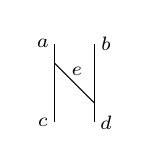
\begin{tikzpicture}[baseline={([yshift=-20pt]current bounding box.north)}]
\draw (0,0) to (0,1);
\draw (0.5,0) to (0.5,1);
\draw (0.5,0.25) to (0,0.75);
\node[font=\fontsize{7}{0}\selectfont] at (-0.15,0) {$c$};
\node[font=\fontsize{7}{0}\selectfont] at (-0.15,1) {$a$};
\node[font=\fontsize{7}{0}\selectfont] at (0.65,0) {$d$};
\node[font=\fontsize{7}{0}\selectfont] at (0.65,1) {$b$};
\node[font=\fontsize{7}{0}\selectfont] at (0.28,0.65) {$e$};
\end{tikzpicture}
\!\!=\sum_f F^{ab,e}_{cd,f}\!
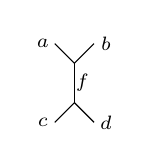
\begin{tikzpicture}[baseline={([yshift=-20pt]current bounding box.north)}]
\draw (0,0) to (0.25,0.25);
\draw (0.5,0) to (0.25,0.25);
\draw (0.25,0.25) to (0.25,0.75);
\draw (0.25,0.75) to (0,1);
\draw (0.25,0.75) to (0.5,1);
\node[font=\fontsize{7}{0}\selectfont] at (-0.15,0) {$c$};
\node[font=\fontsize{7}{0}\selectfont] at (-0.15,1) {$a$};
\node[font=\fontsize{7}{0}\selectfont] at (0.65,0) {$d$};
\node[font=\fontsize{7}{0}\selectfont] at (0.65,1) {$b$};
\node[font=\fontsize{7}{0}\selectfont] at (0.35,0.5) {$f$};
\end{tikzpicture}\quad , \quad
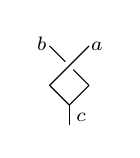
\begin{tikzpicture}[baseline={([yshift=-20pt]current bounding box.north)}]
\draw (0,0) to (0,0.25);
\draw (0,0.25) to (0.25,0.5);
\draw (0.25,0.5) to (0.05,0.7);
\draw (-0.05,0.8) to (-0.25,1);
\draw (0,0.25) to (-0.25,0.5);
\draw (-0.25,0.5) to (0.25,1);
\node[font=\fontsize{7}{0}\selectfont] at (0.15,0.1) {$c$};
\node[font=\fontsize{7}{0}\selectfont] at (0.35,1) {$a$};
\node[font=\fontsize{7}{0}\selectfont] at (-0.35,1.03) {$b$};
\end{tikzpicture}
\!\!=R^{ab}_{c}\!
\begin{tikzpicture}[baseline={([yshift=-20pt]current bounding box.north)}]
\draw (0,0) to (0,0.5);
\draw (0,0.5) to (0.25,1);
\draw (0,0.5) to (-0.25,1);
\node[font=\fontsize{7}{0}\selectfont] at (0.15,0.1) {$c$};
\node[font=\fontsize{7}{0}\selectfont] at (0.35,1.02) {$b$};
\node[font=\fontsize{7}{0}\selectfont] at (-0.35,1) {$a$};
\end{tikzpicture}.
\end{equation*}


These manipulations encode the data of the unitary modular tensor category, and can be used to represent the state of a system of anyons as a linear combination of fusion trees. For the Fibonacci anyons, the non-trivial $R$ and $F$ moves are given by
\begin{align}
	R_{\mathbb{I}}^{\tau\tau}&= \e^{\frac{-4\pi i}{5}}\qquad R_\tau^{\tau\tau}= \e^{\frac{3\pi i}{5}}\\
	F_{\tau}^{\tau\tau\tau} &= \begin{pmatrix}\varphi^{-1}&\varphi^{-\frac{1}{2}}\\\varphi^{-\frac{1}{2}}&-\varphi^{-1}\end{pmatrix} \,,
\end{align}
where in the last expression, $\varphi=\frac{1+\sqrt{5}}{2}$ is the golden ratio, and the matrix is given in a basis labelled $(\mathbb{I},\tau)$.

We use a phenomenological model of Fibonacci anyon dynamics which neglects any 
microscopic details of the system. 
This is consistent with the principles of topologically 
ordered systems and anyonic physics, where the key universal features describing the 
anyon model correspond to large length-scale physics, while the microscopic physics plays 
a less important (and non-universal) role.
We simulate a $(2+1)$-dimensional topological quantum field theory.
%Effectively, we simulate a $(2+1)$-dimensional topological quantum field theory on a discrete space-time.
%As such, we model the system simply as a 
%periodic $L\times L$ square lattice $\Lambda$ of sites upon which sets of anyons can 
%reside. 
%Allowed anyon dynamics (pair-creation, braiding, and fusion) are considered to act 
%locally on edges of $\Lambda$. 
%For more details of an analogous model, see~\cite{Brell2013}.
\dude{something about observables vs. states.}

%------------------------------------------------------------------------------------------------------------%
\paragraph{Noise and error-correction.}

We consider encoding a qubit of quantum information in the global degeneracy associated 
with the topology of the manifold of our system. We imagine an idealized Hamiltonian for this 
system of the form
\begin{align}
	H=-\sum_{i\in \Lambda}\proj{\mathbb{I}}_i\;,\label{e:hamiltonian}
\end{align}
with $\proj{\mathbb{I}}_i$ the projector to charge $\mathbb{I}$ at site $i$, i.e.~the ground 
space of the model has vacuum (or no anyon) at each site. Given the toroidal boundary 
conditions, this space is two-fold degenerate as noted above. We identify this ground space 
as the codespace of our model. Typical realistic noise processes in this kind of system are 
pair-creation, hopping, exchange etc.~of anyons on neighboring sites of $\Lambda$. It was 
seen in~\cite{Brell2013} that a simplified noise model consisting of pair-creation events only 
is sufficient to capture the qualitative features of an error-correction simulation, and so for convenience we 
will restrict to pair-creation noise processes in the numerical results presented in this study. 
Such pair-creation events act on neighboring pairs of sites,
and so may be associated with an edge of the lattice, chosen 
uniformly at random at each time step of the simulation. The simulation time, and thus the 
error-correction threshold, will be measured in terms of average number of noise processes 
per edge, as opposed to an iid noise probability per edge. The latter measure is not 
appropriate for error processes in nonabelian anyon models, but the two coincide in the limit 
of low error rates in those cases where they are comparable (see Ref.~\cite{Brell2013}).

In order to perform a logical error on our code, a noise process must have support on a 
ribbon running around a homologically nontrivial loop of the lattice. These correspond to 
processes in which anyonic charge is transported around the non-trivial loop before 
annihilating to vacuum.
% cggb{we want to define logical operators as those that map the codespace to itself, so for it to be a logical operator, they must annihilate to vacuum. they need not be unitary}.

Our error-correction algorithm is
based on a heirarchical clustering algorithm~\cite{Hastie2009},
and has some 
similarities to the hard-decision renormalization group (RG) decoder~\cite{Bravyi2011}. 
The decoder proceeds by measuring the occupations of 
anyons at each site of the lattice, forming clusters of nearby anyons and 
%fusing the anyons within each cluster. 
measureing the total charge within each cluster.
Clusters with trivial charge are discarded, and
the rest are joined (agglomeratively~\cite{Hastie2009})
at linearly increasing length scales.
See FIG. \ref{f:decode}.
Note that unlike the abelian case, the decoder
cannot know the charge of each cluster based only
on the syndrome information (as in \cite{Bravyi2011}),
and so will query (measure) the system to find this.
The simulation proceeds in this way as a dialogue between decoder
and system, terminating when the lattice 
is free of anyons (i.e.~we have returned to the codespace) 
or the decoder performs a homologically nontrivial operation, thereby altering the codespace.
%or the clustering length scale exceeds the size of the lattice.
%\cggb{our simulation may terminate when the decoder performs a nontrivial operation, but here we're just describing the decoder, which can't know that.}
%\dude{in our sim the decoder stops when there is one cluster. Ie., it never gives up.}
%\cggb{A few more details? What is our length schedule?} 
%\cggb{How does our decoder relate to other decoding schemes used in~\cite{Wootton2013,Brell2013,Hutter2014}?} 
Note that, as was found in Ref.~\cite{Brell2013}, we expect that our qualitative results may be reproduced by most alternative families of decoders, although it may not be clear in all cases how to extend these decoders to the non-abelian setting.
The advantage of using a hard-decision decoder is 
its simplicity and flexibility, and the fact that its clustering scheme is compatible with the structure in the noise processes that allows us to classically simulate them.

\begin{figure}[th!]
\begin{center}
	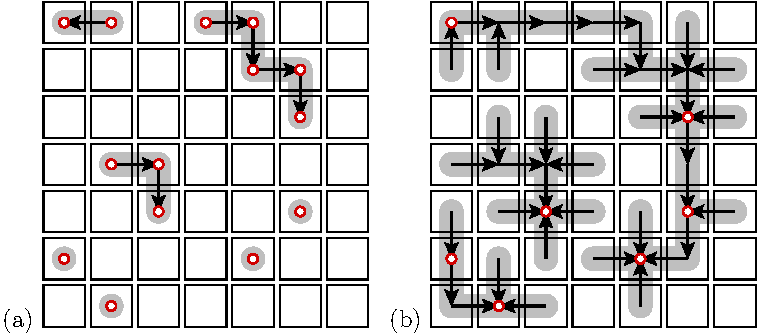
\includegraphics[width=1.0\columnwidth]{pic-decode.pdf}
\caption{The decoder works by maintaining a set of disjoint clusters as rooted trees.
(a) Trees are formed from neighboring sites that contain a charge.
(b) For each successive round, we grow all trees, 
and overlapping trees are joined to form
a single tree. Arrows denote movement of charge to the root of the tree.
The root of each tree is chosen arbitrarily.
}
\label{f:decode}
\end{center}
\end{figure}

%\begin{figure*}[th!]
%\begin{center}
%	{\scriptsize (a)
%	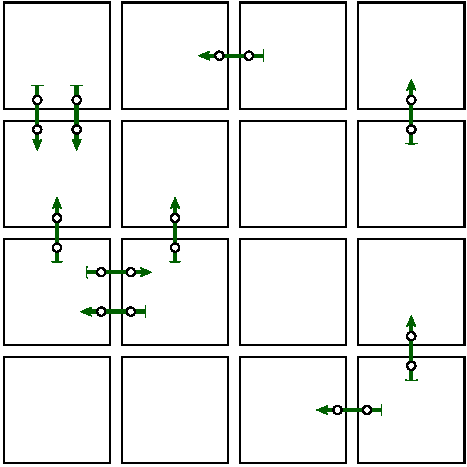
\includegraphics[width=0.45\columnwidth]{pair-create.pdf}
%	\hskip 4pt
%	(b)
%	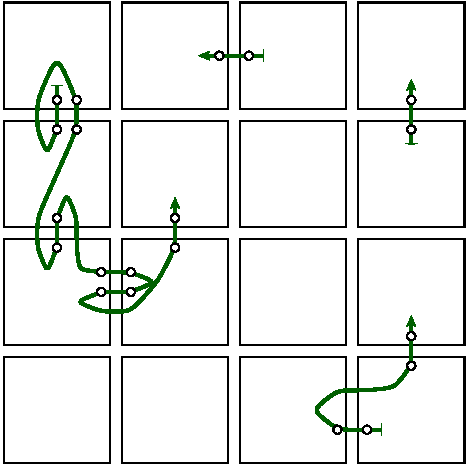
\includegraphics[width=0.45\columnwidth]{syndrome-1.pdf}
%	\hskip 4pt
%	(c)
%	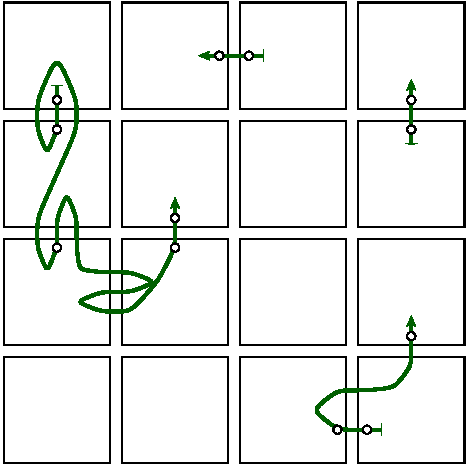
\includegraphics[width=0.45\columnwidth]{syndrome-2.pdf}
%	\hskip 4pt
%	(d)}
%	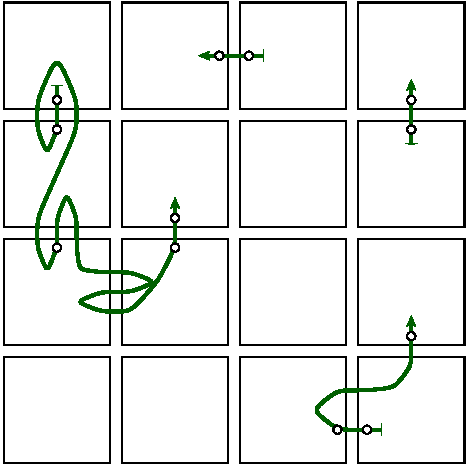
\includegraphics[width=0.45\columnwidth]{syndrome-2.pdf}
%\caption{\stf{polish this a bit} The simulation of noise processes proceeds by a) creating pairs of anyons on neighboring tiles represented by open curves b) joining the curves within a given tile c) measuring the total charge on each tile. \stf{Add another graph that shows how we use syndrome info.}}
%\label{f:simex}
%\end{center}
%\end{figure*}

%------------------------------------------------------------------------------------------------------------%	
\paragraph{Classical simulability.}

Although simulating pair creation, braiding, and fusion of $n$ Fibonacci anyons is equivalent 
in computational power to universal quantum computing (and thus unlikely to be classically 
tractable), noise processes and error-correction procedures have structure that we can 
exploit to efficiently simulate typical processes of interest. In particular, those 
processes in which we expect error-correction to succeed are also those that we expect to 
be able to efficiently simulate for the following heuristic reasons (we leave a more rigorous analysis of simulability for noise and error correction processes as an open problem).

Below the (bond) percolation threshold for (say) a 2D square lattice, we expect random sets of 
bonds to decompose into separate clusters~\footnote{
We use the word cluster to refer both to groupings 
of nearby anyons as formed by the decoding algorithm and 
to connected components of a graph under percolation\dude{confusing}, since both 
of these usages are standard in the literature. The intended 
meaning will remain clear from context.} of average size $O(\log(n))$ and variance 
$O(1)$~\cite{Bazant2000}.
Each noise process in our model is associated with a (randomly distributed) edge, and so 
disconnected clusters correspond to sets of anyons that could not have interacted at any 
point in their history. 
Although normally anyons can interact by braiding without ever coming 
into contact with one another \dude{um um um}, in this case charge conservation 
implies that each distinct cluster must have trivial total charge, and so all such interactions are trivial.
This allows us to simulate the braiding processes within each cluster 
separately. In other words: the quantum state in the fusion space of all anyons factorizes into 
a tensor product over bond clusters, and we can compute each factor separately. Since each 
cluster has size only $O(\log(n))$, we can typically simulate these dynamics efficiently 
because the resulting fusion space has dimension $O(\mathrm{poly}(n))$. There are rare 
random processes that violate this reasoning, but processes such as these are suppressed 
exponentially in the lattice size $L$~\cite{Grimmett1989}. 

However, random noise processes are not the only dynamics that we need to consider. We 
must also consider the effect of the error-correction routine itself. This acts iteratively to fuse 
particles on increasing length scales. While this kind of fusion would typically merge clusters, 
forcing us to compute dynamics of larger and larger sets of anyons, large clusters are sparsely distributed 
(and thus unlikely to be merged), and in addition at each length scale the total number of 
anyons present is dramatically reduced by fusion, leading to a smaller number of anyons that 
must be simulated.

Of course, if we were to consider noise so strong that 
the clusters percolate over the entire lattice, we would no 
longer expect to be able to efficiently simulate the noise and recovery processes in the system. 
However, recall that logical errors in our system correspond to processes that act over a non-trivial loop of the torus. 
Our simulation remains efficient \dude{efficiency has nothing to do with it}
until the point that we start to create nontrivial loops around the torus, 
and our simulation begins to declare failure whenever non-trivial logical 
operations occur, meaning that we can simulate large lattice sizes 
in the successful error-correction (sub-percolated) regime, including up to $L=128$.

%------------------------------------------------------------------------------------------------------------%	
\paragraph{Simulation algorithm.}

%\stf{Add figure about observables versus states.}

Our concrete simulation proceeds by associating a \emph{tile} with each site of the 
$L\times L$ periodic square lattice.
In order to keep track of the observables of the system 
we maintain a set of disjoint curves, representing the history of anyons on the lattice.
These curves can also be thought of as a top-down view of the fusion tree:
the anyons comprising the fusion tree are here displayed as points along each curve. 
In general, the curves wind around the two 
dimensional tiles in a haphazard way determined by the progress of the simulation.
This allows a dynamically generated basis for the fusion space that easily allows for tensor 
decomposition into factors corresponding 
to disjoint clusters \dude{confusing use of this word}.
For comparison, previous work 
used a single fixed basis for the fusion space (determined by row-major ordering of 
sites)~\cite{Brell2013}.


\begin{figure}[th!]
\begin{center}
	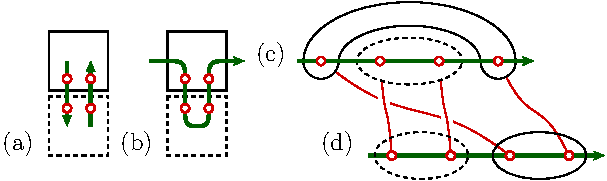
\includegraphics[width=1.0\columnwidth]{pic-syndrome.pdf}
\caption{Four equivalent representations of a state,
along with two syndrome observables marked with solid and dashed lines:
(a) two pairs are joined in (b).
Deform the curve straight to get (c),
then effect some
braid operations on the state so that (d) the two
observables are now represented on the curve. 
%\cggb{I'm not totally clear on what I'm looking at here. Is this the diagram where we want to explain the whole simulation algorithm? Is the idea that we start with a), which is given by the set of noise processes that have happened, then we connect stuff up arbitrarily into b) to make some fusion tree. Then c) is what's happening after linearizing the picture? And d) is c) after some R and F moves so you go into the standard basis for the fusion tree? Are the red lines between c) and d) just denoting leaves with the same identity or do they have some more precise meaning wrt the braid moves that relate c) and d)?}
}
\label{f:syndrome}
\end{center}
\end{figure}

In FIG. \ref{f:syndrome} we show two adjacent sites
involved in a syndrome measurement.
%This will be the total charge on each site, ie. either $\tau$ or $\mathbb{I}.$
The error process has resulted in two pair
creation events along the edge joining these sites.
\dude{i'd like to write out the equations for each of
these 4 steps, but we'd need to keep it tight somehow.}
First, (a) we show the state as a tensor product of two pairs $\tau\tau\otimes\tau\tau$.
Then, (b) these two pairs are embedded into a single larger fusion
tree $\tau\tau\tau\tau$.
This is continuosly deformable into the picture in (c).
It is now clear the two braid operations required so
that the observables are represented on the fusion tree.
The general algorithm and datastructures used
for this proceedure will be discussed elsewhere.

\dude{Arrgh, what do we say about how to simulate moving anyons around
the lattice ?}

%Each round of simulation proceeds in four steps as follows (an example is shown 
%in \Fref{f:simex}).
%
%\begin{enumerate}[a)]
%\item The noise process is modeled by a sequence of pair-creation events distributed as 
%a Poisson process across each edge. Curves are created crossing the relevant edge 
%and terminating on the neighboring sites.
%\item We first join curves that participate in the same tile in order to, 
%\cggb{maybe a couple more lines of detail on this and the next point? perhaps also the previous paragraph?}
%\item measure the charge on each tile. Any resulting anyon is left somewhere in the tile.
%\item The decoder examines this syndrome and clusters nearby anyons. Each cluster 
%is then measured (fused), and the decoder continues to cluster and fuse on larger 
%scales until there are no more anyons, or a cluster includes a non-trivial loop on the 
%lattice. Since operators with support on such non-trivial clusters will generally perform an 
%undetectable error on the encoded state, in this case we abandon the simulation and 
%declare failure to error correct.
%\end{enumerate}

\stf{Cite~\cite{Pfeifer2010} for braiding tricks}

%------------------------------------------------------------------------------------------------------------%
\paragraph{Numerical results.}

We plot the performance of the decoder as a function of error rate for varying lattice sizes in 
\Fref{f:threshold}. 
The error rate is parameterized by the Poisson process duration $t_{\mathrm{sim}}$, representing the expected number of errors per edge during the simulation. 
We find evidence of a decoding threshold below which decoding succeeds with asymptotic 
certainty as the system size increases at $t_{\mathrm{sim}}\simeq 0.125 \pm 0.003$.

\begin{figure}[th!]
\begin{center}
	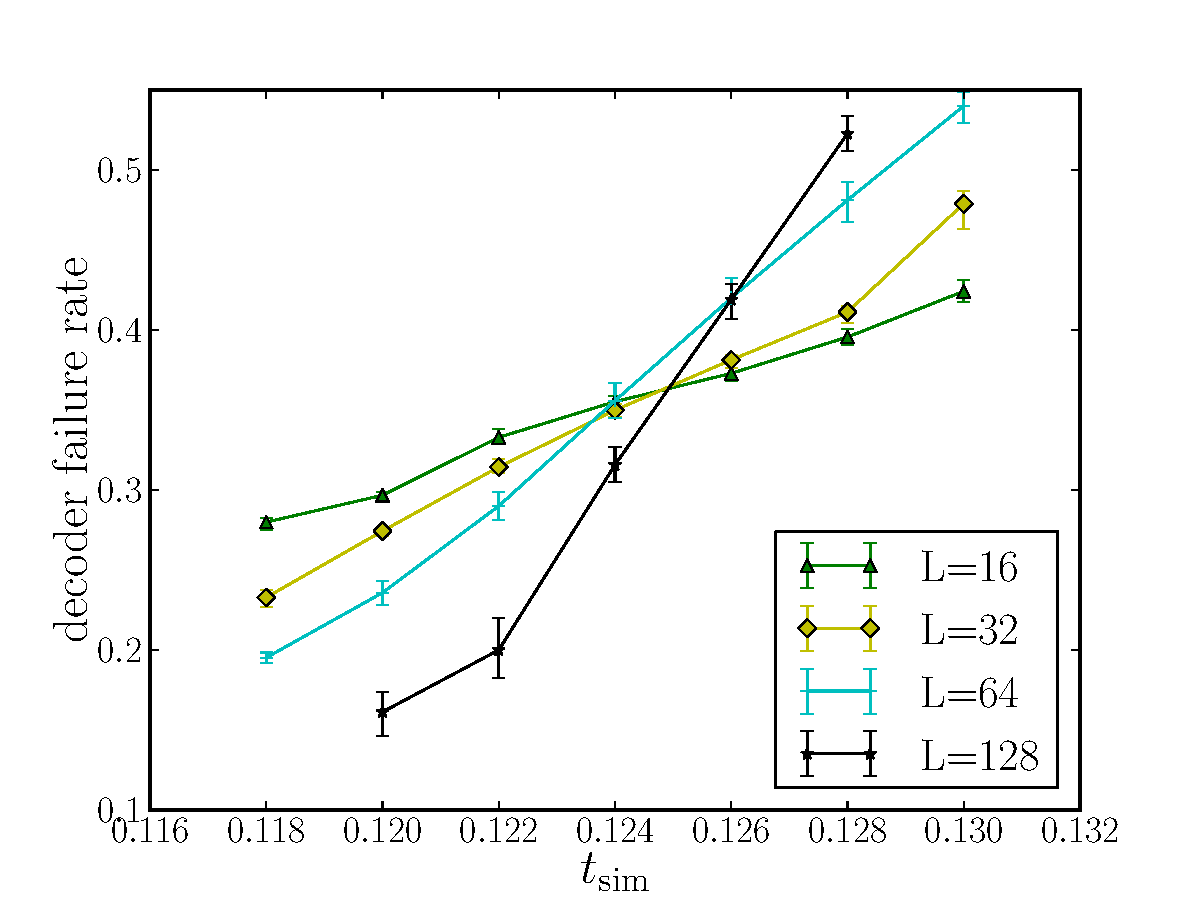
\includegraphics[width=\columnwidth]{anyons-kyle.pdf}
\caption{\stf{polish this a bit} Decoder failure as a function of simulation time for various lattice sizes, showing 
threshold behavior at around $t_{\mathrm{sim}}\simeq 0.125$.}
\label{f:threshold}
\end{center}
\end{figure}

We can guarantee that error-correction will succeed whenever noise does not percolate, but it is possible that percolated events may still result in no error. 
The connection between the percolation threshold and the error-correction threshold is not well understood in general~\cite{Hastings2014}, though it is clear that our threshold estimate will be a lower bound for the true threshold that may be found if all events (including those that have percolated) were simulated by an optimal decoder. 
However, calculations of such nontrivial operations suggest that all such processes will indeed result in a logical or leakage error.
As such it is likely that neglecting full simulation for such events does not significantly affect our observed threshold value.

%------------------------------------------------------------------------------------------------------------%
\paragraph{Discussion.}

We have demonstrated classical simulation of successful error correction in a universal anyon model. 
Though we have chosen several properties of our model and simulation in a convenient way for simplicity, it seems highly unlikely that they will affect the qualitative results, similarly to the results of Ref.~\cite{Brell2013}. 
In particular, although we have modeled our logical qubit as encoded in the global topological degrees of freedom of our system, we could have encoded it in the fusion space of several preferred $\tau$ anyons. 
This situation would be appropriate to model error-correction routines for topological quantum computation. 
Additionally, we expect our results to be stable to changes in details of the noise model and decoding algorithm.

None of our techniques are restricted to simulation of Fibonacci anyon dynamics, and could 
equally well be used to simulate successful error-correction protocols in an arbitrary anyon 
code. 
As such, our methods could be used to demonstrate successful error-correction in an arbitrary anyonic topological quantum computation.

There are several interesting avenues for further research. 
Although it is not completely obvious how to do so, applying these methods to more realistic models such as concrete microscopic spin models or models with non-topological features would give direct insight into practical error rates needed for topological quantum memories in non-Abelian systems. 
Another potential direction is to incorporate tensor network methods for simulating anyons~\cite{Pfeifer2012, Singh2014} to improve the speed and scale of the simulations. 
Finally, perhaps the most important open question is whether \emph{fault-tolerant} decoders can be designed for nonabelian anyon codes. 


%------------------------------------------------------------------------------------------------------------%
\acknowledgments 

We thank A.\ Doherty and R.\ Pfeifer for discussions. 
This work was supported by the ARC via EQuS project number CE11001013, by the US Army Research Office grant numbers W911NF-14-1-0098 and W911NF-14-1-0103, ERC grant QFTCMPS and by the cluster of excellence EXC 201 Quantum Engineering and Space-Time Research. STF also acknowledges support from an ARC Future Fellowship FT130101744.

%------------------------------------------------------------------------------------------------------------%
\bibliography{refs2}

\end{document}
